\documentclass[tikz,border=8pt]{standalone}
\usepackage{amsmath,amssymb}
\usetikzlibrary{arrows.meta,automata,positioning,quotes}
\begin{document}
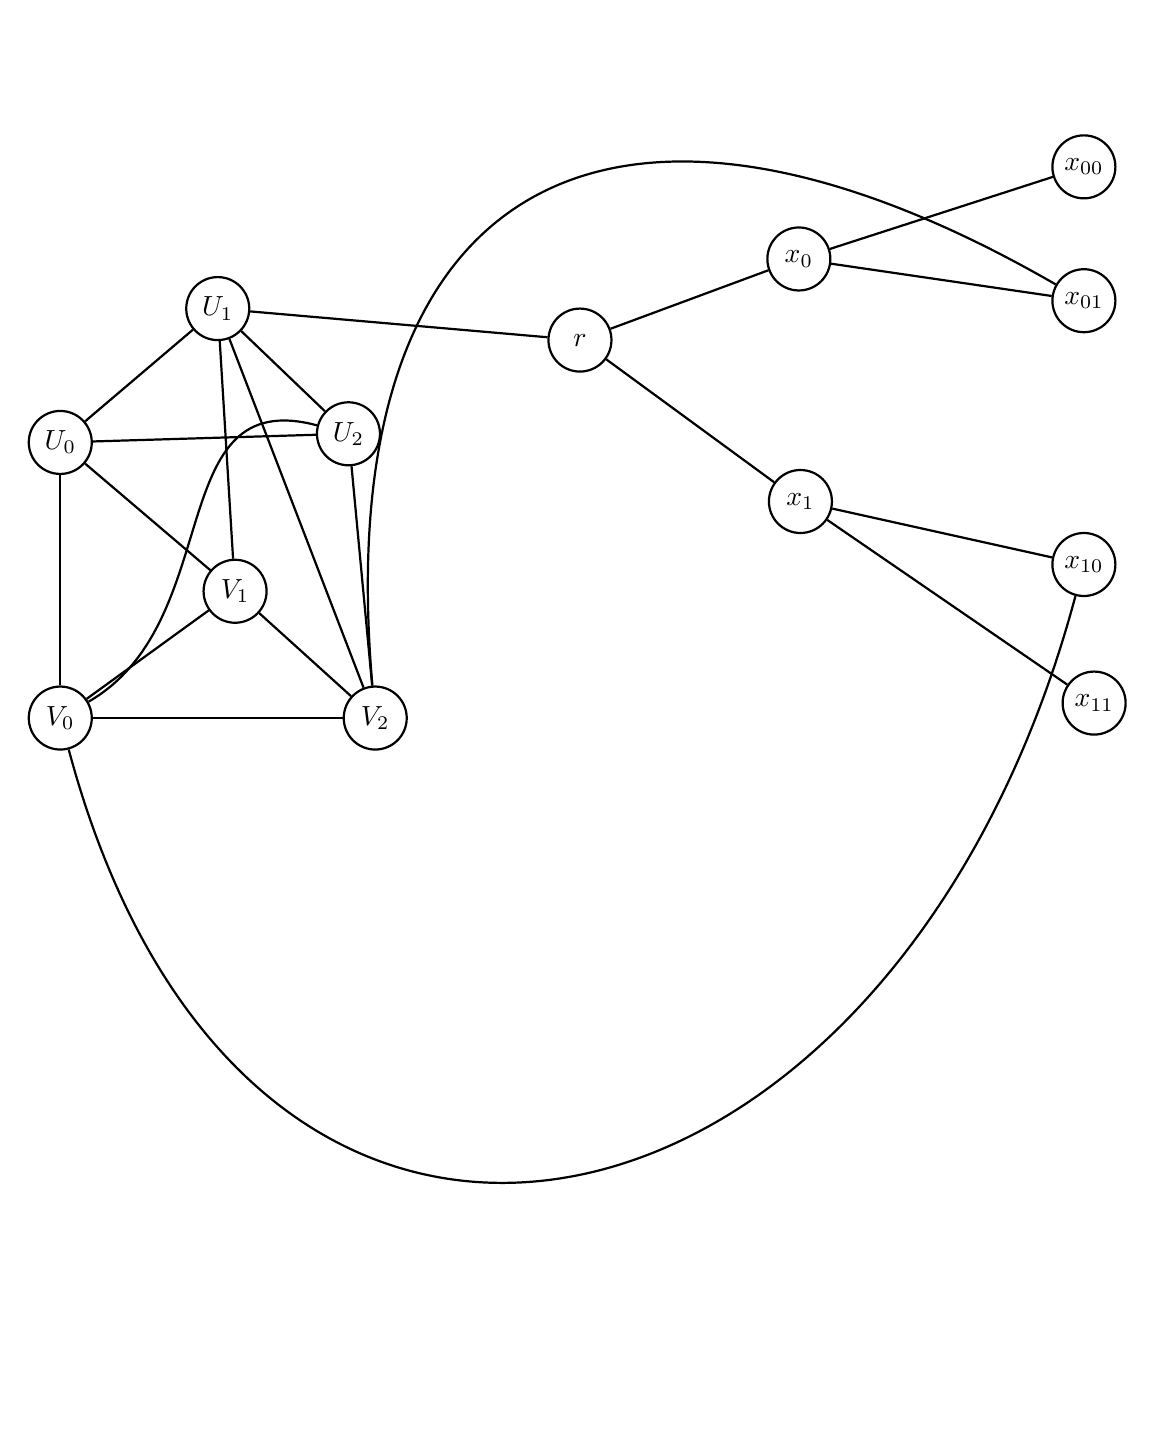
\begin{tikzpicture}[x=1cm,y=1cm]
\tikzset{
  graphnode/.style={circle,draw,thick,minimum size=8mm,inner sep=1pt,font=\sffamily},
  directed/.style={-{Stealth[length=2.4mm]},thick},
  undirected/.style={thick}
}
\node[graphnode] (n_U0) at (-6.20,2.20) {$U_0$};
\node[graphnode] (n_U1) at (-4.20,3.90) {$U_1$};
\node[graphnode] (n_U2) at (-2.54,2.31) {$U_2$};
\node[graphnode] (n_V0) at (-6.20,-1.30) {$V_0$};
\node[graphnode] (n_V1) at (-3.98,0.31) {$V_1$};
\node[graphnode] (n_V2) at (-2.20,-1.30) {$V_2$};
\node[graphnode] (n_r) at (0.40,3.50) {$r$};
\node[graphnode] (n_x0) at (3.18,4.53) {$x_0$};
\node[graphnode] (n_x1) at (3.20,1.45) {$x_1$};
\node[graphnode] (n_x00) at (6.80,5.70) {$x_{00}$};
\node[graphnode] (n_x01) at (6.80,4.00) {$x_{01}$};
\node[graphnode] (n_x10) at (6.80,0.65) {$x_{10}$};
\node[graphnode] (n_x11) at (6.93,-1.11) {$x_{11}$};
\draw[undirected] (n_U0) -- (n_U1);
\draw[undirected] (n_U1) -- (n_U2);
\draw[undirected] (n_U0) -- (n_U2);
\draw[undirected] (n_V0) -- (n_V1);
\draw[undirected] (n_V1) -- (n_V2);
\draw[undirected] (n_V0) -- (n_V2);
\draw[undirected] (n_U0) -- (n_V0);
\draw[undirected] (n_U1) -- (n_V1);
\draw[undirected] (n_U2) -- (n_V2);
\draw[undirected] (n_U0) -- (n_V1);
\draw[undirected] (n_U1) -- (n_V2);
\draw[undirected] (n_U2) to[out=165,in=30,looseness=1.15] (n_V0);
\draw[undirected] (n_U1) -- (n_r);
\draw[undirected] (n_r) -- (n_x0);
\draw[undirected] (n_r) -- (n_x1);
\draw[undirected] (n_x0) -- (n_x00);
\draw[undirected] (n_x0) -- (n_x01);
\draw[undirected] (n_x1) -- (n_x10);
\draw[undirected] (n_x1) -- (n_x11);
\draw[undirected] (n_V2) to[out=95,in=150,looseness=1.65] (n_x01);
\draw[undirected] (n_V0) to[out=-75,in=-105,looseness=1.75] (n_x10);
\end{tikzpicture}
\end{document}
